\documentclass[review]{elsarticle}

\usepackage{amsmath,amssymb}
\usepackage{graphicx}
\usepackage{booktabs}
\usepackage{multirow}
\usepackage{lineno}
\usepackage[margin=2.5cm]{geometry}
\usepackage{hyperref}

\journal{Thermal Science and Engineering Progress}

\begin{document}

\begin{frontmatter}

\title{Multi-Mechanism Pre-Training of Physics-Informed Neural Networks for Fouling Resistance Reconstruction from Sparse Measurements}

% Author details removed for double-blind review.
% Full title page with author information is provided as a separate file.

\begin{abstract}
Heat exchanger fouling is a major source of energy loss in the process industry, yet accurate estimation of fouling resistance evolution $R_f(t)$ is hindered by severe data scarcity in practical settings. This study proposes a multi-mechanism pre-training framework that leverages five distinct fouling ODE models to pre-train a Physics-Informed Neural Network (PINN) on diverse synthetic data, followed by parameter-efficient fine-tuning on extremely sparse real measurements ($N = 5$--$30$ points). We validate the framework on 18 fouling curves digitized from three peer-reviewed studies, spanning crystallization fouling, crude oil fouling, and CaCO$_3$ precipitation with induction periods. A critical baseline reveals that direct ODE curve fitting fails on 15 of 18 curves with sparse data ($R^2 \approx 0$ or negative), while PINN pre-training rescues 12 of these failures. For pure interpolation, smoothing spline and Gaussian Process baselines remain highly competitive with the PINN (median $R^2 \approx 0.99$ at $N=15$; see Supplementary Table~S2); the principal value of the proposed framework lies in physics-grounded representation and downstream decision integration rather than universal interpolation superiority. Key findings include: (1) multi-mechanism pre-training provides gains beyond data volume---when matched for trajectory count (2,000 each), single-mechanism pre-training achieves $R^2 = 0.62$ on its target curve type, while multi-mechanism pre-training reaches $R^2 = 0.91$ (+0.29 gain from mechanism diversity, not data volume); at lower volume (200 trajectories), single-mechanism pre-training collapses to $R^2 = -1329$, illustrating that both volume and diversity matter; (2) the framework achieves mean $R^2 > 0.90$ on 12 of 18 curves with only 15 training points in 5-seed multi-seed validation; (3) the pre-trained PINN outperforms Random Forest in extrapolation on 6 of 8 tested curves at $N=5$ (median $\Delta R^2 = +1.8$), though both methods produce negative absolute $R^2$---extrapolation remains an open challenge for all methods; and (4) in a retrospective illustrative cleaning analysis, PINN-derived schedules produced 20--67\% lower dimensionless cost ratios than fixed-interval policies on curves with reliable reconstruction accuracy ($R^2 > 0.80$), with strategy rankings stable across a four-level threshold sensitivity analysis. Pre-training uses only publicly available physics models. Fine-tuning on a target curve takes approximately 3 seconds on consumer GPU hardware---though the current pipeline requires a human to select the appropriate ODE model based on curve morphology; an N-point-only geometric auto-selector achieves 87\% accuracy (Supplementary Table~S1), demonstrating feasibility for automation.
\end{abstract}

\begin{keyword}
Physics-Informed Neural Networks \sep heat exchanger fouling \sep sparse data \sep transfer learning \sep cleaning optimization \sep multi-mechanism modeling
\end{keyword}

\end{frontmatter}

\linenumbers

%=====================================================================
\section{Introduction}
%=====================================================================

\subsection{Problem Background}

Heat exchangers are ubiquitous in the chemical, petroleum, power generation, and food processing industries. During operation, dissolved salts (CaCO$_3$, CaSO$_4$), particulates, and organic compounds deposit on heat transfer surfaces, forming a fouling layer whose thermal conductivity (0.5--2 W/m$\cdot$K) is one to two orders of magnitude lower than that of the metal tube wall (50--400 W/m$\cdot$K) \cite{muller2005fouling}. The resulting increase in overall thermal resistance forces plants to either increase driving temperature differences (and thus fuel consumption) or accept reduced throughput.

The fouling thermal resistance $R_f(t)$ evolves according to the net effect of deposition and removal processes:
\begin{equation}
\frac{dR_f}{dt} = \phi_d - \phi_r
\end{equation}
where $\phi_d$ is the deposition rate and $\phi_r$ is the removal rate---both functions of local temperature, velocity, concentration, and surface conditions.

\subsection{The Cleaning Decision Problem}

Since fouling is unavoidable, industrial practice relies on periodic cleaning to restore heat transfer efficiency. The cleaning scheduling problem is an optimization: clean too frequently and incur excessive downtime costs; clean too infrequently and suffer escalating energy penalties. The optimal cleaning interval minimizes the sum:
\begin{equation}
\min_{t_{\text{clean}}} \left[ \text{Energy Penalty}(t_{\text{clean}}) + \text{Cleaning Cost} + \text{Downtime Cost} \right]
\end{equation}
This optimization requires accurate reconstruction of $R_f(t)$ from sparse measurements, specifically the time at which the fouling resistance will exceed a critical threshold $R_{f,\text{crit}}$. Without a reliable predictive model, cleaning decisions are made by heuristics---typically fixed calendar intervals---that are almost certainly suboptimal.

\subsection{The Data Scarcity Problem}

Accurate $R_f(t)$ estimation faces a fundamental obstacle: industrial fouling data is extremely scarce. Plant operators are reluctant to share operational data due to competitive sensitivity, and installing dedicated fouling monitoring instrumentation is expensive. The typical industrial scenario involves a handful of historical cleaning records and occasional temperature/pressure measurements convertible to $R_f$ estimates.

Standard machine learning approaches (MLPs, random forests, gradient boosting) require hundreds to thousands of labeled examples to achieve acceptable accuracy. With only 5--30 data points---the realistic industrial scenario---purely data-driven methods either fail completely or produce physically implausible predictions.

\subsection{PINNs as a Solution and Their Limitations}

Physics-Informed Neural Networks (PINNs) \cite{raissi2019physics} address data scarcity by augmenting the standard data loss with a physics-based regularization term:
\begin{equation}
\mathcal{L} = \underbrace{\text{MSE}(R_f^{\text{pred}} - R_f^{\text{obs}})}_{\text{Data Loss}} + \lambda \cdot \underbrace{\text{MSE}\left(\frac{dR_f}{dt} - (\phi_d - \phi_r), 0\right)}_{\text{Physics Loss}}
\end{equation}
The physics loss enforces the governing ODE at collocation points where no observational data is available, effectively providing an infinite source of ``free'' training signal \cite{karniadakis2021physics}.

However, existing PINN approaches for fouling suffer from two critical limitations: (1) they use only the Kern-Seaton asymptotic model as the physics constraint, while real fouling exhibits diverse mechanisms---induction periods, threshold behavior, cleaning-induced discontinuities; and (2) all experiments to date have been conducted on synthetic data generated by the same model used in the physics loss, creating a self-consistency loop where the PINN is merely learning to invert a known equation rather than discovering genuine physical structure.

\subsection{Contributions of This Work}

This study addresses both limitations through a multi-mechanism pre-training framework. Our specific contributions are:

\begin{enumerate}
\item \textbf{Multi-mechanism ODE registry}: We implement five distinct fouling ODE models with a unified interface, enabling PINN pre-training on diverse synthetic fouling physics.
\item \textbf{Pre-training + fine-tuning pipeline}: We demonstrate that pre-training a PINN on multi-mechanism synthetic data creates a physics-informed prior that transfers to real fouling curves via lightweight fine-tuning on as few as 5--30 sparse data points.
\item \textbf{Comprehensive real-data validation}: We digitize and validate on 18 real fouling curves from three independent experimental studies, covering three fouling types and multiple surface conditions.
\item \textbf{Single vs.\ multi-mechanism ablation}: Using a KS-large control (2,000 trajectories, matching multi-mechanism volume), we disentangle data volume from mechanism diversity. Multi-mechanism pre-training outperforms single-mechanism by $\Delta R^2 = +0.29$ at equal volume, and both substantially outperform the low-volume single-mechanism baseline ($R^2 = -1329$ at 200 trajectories). Both data volume and mechanism diversity contribute independently to pre-training quality.
\item \textbf{ODE-fit baseline and honest assessment}: By comparing against direct ODE curve fitting, we show that pure physics models fail on 15 of 18 curves with sparse data, precisely identifying the regime where PINN pre-training provides value---and honestly acknowledging where simpler methods suffice.
\end{enumerate}

%=====================================================================
\section{Methodology}
%=====================================================================

\subsection{Multi-Mechanism Fouling ODE Registry}

We implement five fouling kinetics models with a unified Python interface. Each model provides an analytical solution $R_f(t)$ (if available) for synthetic data generation and an ODE residual function $\mathcal{R}(dR_f/dt, R_f, \mathbf{p})$ for PINN physics loss computation.

\textbf{Model 1---Kern-Seaton (KS)}: The classical asymptotic fouling model \cite{kern1959theoretical}:
\begin{align}
\frac{dR_f}{dt} &= A \exp\left(-\frac{E_a}{RT_w}\right) - B \cdot \tau_s \cdot R_f \\
R_f(t) &= R_f^*\left(1 - \exp(-t/\tau)\right), \quad R_f^* = \frac{\phi_d}{B\tau_s}, \quad \tau = \frac{1}{B\tau_s} \nonumber
\end{align}
Applicable to: crystallization fouling, particulate fouling with asymptotic behavior.

\textbf{Model 2---KS with Initial Residual}: Extends Model 1 with $R_f(0) = R_{f0} > 0$, modeling incomplete cleaning. Applicable to heat exchangers with residual fouling after chemical cleaning.

\textbf{Model 3---Simplified KS (Phenomenological)}: A 3-parameter form for direct curve fitting:
\begin{equation}
\frac{dR_f}{dt} = \frac{R_f^* - R_f}{\tau}, \quad R_f(t) = R_{f0} + R_f^*(1 - e^{-t/\tau})
\end{equation}
Applicable to all asymptotic curves with unknown physical parameters.

\textbf{Model 4---Induction + Linear Growth}: Models the characteristic delay before rapid fouling onset:
\begin{equation}
R_f(t) = \begin{cases} 0 & t < t_{\text{ind}} \\ k_{\text{growth}} \cdot (t - t_{\text{ind}}) & t \geq t_{\text{ind}} \end{cases}
\end{equation}
The analytical form is piecewise-defined and non-differentiable at $t = t_{\text{ind}}$. For PINN physics loss computation, we use a smoothed approximation with a sigmoid function (slope $\alpha = 10$) providing a continuous transition. The analytical solution used for data generation and curve fitting uses the exact piecewise form. Applicable to CaCO$_3$ crystallization on modified surfaces.

\textbf{Model 5---Ebert-Panchal Threshold}: Incorporates a critical shear stress below which fouling does not occur \cite{ebert1997analysis}:
\begin{equation}
\frac{dR_f}{dt} = \alpha \cdot \text{Re}^\beta \cdot \text{Pr}^{-0.66} \cdot \exp\left(-\frac{E_a}{RT_{\text{film}}}\right) - \gamma \cdot \tau_w
\end{equation}
Applicable to crude oil fouling with threshold velocity/temperature conditions.

\subsection{PINN Architecture}

The PINN takes a unified 10-dimensional input vector:
\begin{equation}
\mathbf{x} = [t, T_w, v, p_1, p_2, p_3, p_4, p_5, p_6, \text{ode\_type\_id}]^T
\end{equation}
where $p_1$--$p_6$ encode ODE-specific physical parameters and unused slots are zero-filled. The network has 4 hidden layers of 64 neurons each with tanh activation (13,249 parameters). The physics loss is computed per-trajectory using the appropriate ODE residual function from the registry.

\subsection{Pre-training on Multi-Mechanism Synthetic Data}

Pre-training data is generated from all five ODE models with stratified parameter sampling: In-domain (ID) parameters near typical phosphoric acid concentration conditions ($T_w = 340$--380~K, $v = 0.8$--2.5~m/s), Out-of-domain 1 (OOD-1) with shifted parameter ranges, and Out-of-domain 2 (OOD-2) with completely different fouling mechanisms. Each ODE model generates 200 ID + 100 OOD-1 + 100 OOD-2 trajectories (60 time points each, $\sigma = 2 \times 10^{-6}$~m$^2\cdot$K/W Gaussian noise), yielding 2,000 total trajectories. Pre-training runs for 3,000 epochs with mini-batch sampling (8 trajectories per ODE type per epoch), physics loss weight $\lambda = 0.5$, and Adam optimizer with ReduceLROnPlateau scheduling.

\subsection{Sparse Fine-tuning on Real Data}

For each real fouling curve, the fine-tuning pipeline proceeds as:

\begin{enumerate}
\item \textbf{ODE model matching}: Select the appropriate ODE model based on the curve's visual characteristics and the fouling type reported in the source publication. Asymptotic curves (Source 001, Source 002) use Model 3; curves with visible induction periods (Source 003) use Model 4. \textbf{Important caveat}: In the current main experiments, this selection is performed by human annotation using the complete digitized curve, which constitutes information leakage (the annotator sees the full curve that would be unavailable in a real sparse-data setting). To quantify this leakage, we conducted an N-point-only auto-selection ablation using a geometric heuristic operating solely on the $N=15$ sparse points: the ratio of mean $R_f$ in the first third vs.\ last third of sparse observations determines whether an induction period is present (ratio $<0.15 \to$ induction\_linear, otherwise ks\_simple). This auto-selector achieves 87\% accuracy (47/54 trials; full per-trial results in Supplementary Table~S1), and on 13 of 18 curves the ``wrong'' ODE produces $|\Delta R^2| < 0.02$---the pre-training prior partially compensates for mismatched physics constraints. The pipeline is therefore not unduly fragile to this choice, but a robust automated selection method remains necessary for fully hands-off deployment.
\item \textbf{ODE parameter estimation}: Fit the selected ODE model to the $N$ sparse points using \texttt{scipy.curve\_fit}, obtaining estimated physical parameters $\hat{\mathbf{p}}$.
\item \textbf{Condition encoding}: Encode $\hat{\mathbf{p}}$ into the unified 10-dimensional input format.
\item \textbf{Fine-tuning}: Initialize from pre-trained weights, train for 2,000 epochs with $\lambda = 0.3$, learning rate $10^{-4}$, and 150 collocation points along the trajectory's time range.
\item \textbf{Full-curve reconstruction}: Evaluate the fine-tuned model on the complete time range. Note that this evaluates interpolation (training points are randomly scattered across the full range), not forward prediction.
\end{enumerate}

\subsection{Baseline Methods and Ablation Design}

We compare against four baselines: Random Forest (RF, $n=100$ trees), XGBoost ($n=100$, max depth 4), MLP (64-32, with early stopping), and LSTM (single-layer, hidden size 16). Ablation variants (all use the same PINN architecture): Main (PT+Phys)---full method; A1 (NoPT+Phys)---no pre-training, physics loss only; A2 (PT+NoPhys)---pre-trained, data-only fine-tuning; A3 (NoPT+NoPhys)---pure neural network from scratch; and KS-only PT---pre-training with only Kern-Seaton synthetic data (200 trajectories).

\subsection{Real Fouling Curve Dataset}

We digitized 18 real $R_f(t)$ curves from three peer-reviewed studies using WebPlotDigitizer. Table~\ref{tab:dataset} summarizes the data sources.

\begin{table}[htbp]
\centering
\caption{Real fouling curve dataset.}
\label{tab:dataset}
\begin{tabular}{@{}p{2.8cm}p{2.2cm}p{2.2cm}ccp{2.3cm}p{1.5cm}@{}}
\toprule
Source & Fouling Type & System & Curves & Time Range & $R_f$ Range (m$^2\cdot$K/W) & Domain \\
\midrule
Jradi et al.\ (2018) \cite{jradi2018tubular} & Crystallization & Tubular HEX & 1 & 0--102~h & $1.7\!\times\!10^{-6}$--$1.6\!\times\!10^{-4}$ & In-domain \\
Benyahia et al.\ (2014) \cite{benyahia2014study} & Crude oil & Refinery E101 & 2 & 665--733~d & $9.1\!\times\!10^{-4}$--$3.5\!\times\!10^{-3}$ & OOD-1 \\
Riihim\"aki et al.\ (2011) \cite{riihimaki2011crystallization} & CaCO$_3$ & Lab-scale HEX & 15 & 0--84~h & $-5.9\!\times\!10^{-2}$--$2.3\!\times\!10^{-1}$ & OOD-2 \\
\bottomrule
\end{tabular}
\end{table}

The Riihim\"aki et al.\ curves span four experimental configurations: unmodified stainless steel (Fig.\ 4, 3 repeated runs), surface coatings (Fig.\ 5, 3 coatings + reference), surface roughness treatments (Fig.\ 11, grit 80/220 + diamond + reference), and patterned surfaces (Fig.\ 13, flat + 3 patterns). Negative $R_f$ values in the early stages reflect surface roughness effects that temporarily enhance heat transfer before fouling takes over---a well-documented phenomenon in crystallization fouling literature \cite{epstein1983thinking}. We treat these negative values as physically meaningful and do not clip or pre-process them.

\subsection{Evaluation Metrics}

\textbf{Reconstruction accuracy}: $R^2$ and Mean Absolute Error (MAE) on the full curve. Primary results use a fixed random seed (42); Section~\ref{sec:multiseed} reports multi-seed statistics. \textbf{Extrapolation}: Train on the first 50\% of the time range; evaluate on the held-out second 50\% (the full-curve $R^2$ shown includes both seen and unseen regions for completeness, but the metric of interest is extrapolation accuracy on the unseen portion). \textbf{Economic impact}: Dimensionless cost ratio as defined in Section~\ref{sec:economic_model}.

\subsection{Economic Model for Cleaning Optimization}
\label{sec:economic_model}

To quantify the practical benefit of accurate $R_f(t)$ reconstruction, we define a dimensionless cost model. All costs are normalized by the cleaning cost $C_{\text{clean}}$, making the analysis independent of absolute currency units.

\textbf{Cost components}: For a cleaning strategy performing cleanings at times $\{t_1, t_2, \ldots, t_k\}$:
\begin{equation}
C_{\text{total}} = k \cdot C_{\text{clean}} + c_{\text{energy}} \cdot \int_0^T R_f(t) \, dt
\end{equation}
where the integral represents the cumulative energy penalty from fouling-induced heat transfer degradation, proportional to $\int R_f(t) \, dt$ under constant heat duty operation \cite{muller2005fouling}.

\textbf{Cleaning strategies}: Fixed-interval (clean every $T/3$ or $T/4$ days), PINN-predicted (use $\hat{R}_f(t)$ to anticipate threshold crossing at $R_{f,\text{crit}}$, with 10\% safety margin), and Reference threshold policy (uses true $R_f(t)$ to detect threshold crossings---requires perfect real-time fouling monitoring; does \textit{not} minimize total cost and is not a theoretical lower bound).

\textbf{Dimensionless cost ratio}: $\text{Cost Ratio}(S) = C_{\text{total}}(S) / C_{\text{total}}(\text{Reference})$. Ratios below 1.0 indicate that the strategy's cleaning schedule achieves lower total cost than the reference policy's schedule.

\textbf{Threshold definition and sensitivity}: The critical threshold $R_{f,\text{crit}}$ for cleaning depends on the heat exchanger design specification (maximum allowable fouling resistance), which varies by equipment and is unknown to us for the digitized literature curves. As a proxy, we define $R_{f,\text{crit}} = f \cdot \max(R_f)$ and report results for four threshold factors $f \in \{0.50, 0.65, 0.80, 0.95\}$ to assess whether strategy rankings are sensitive to this choice. In industrial practice, the plant engineer would set $R_{f,\text{crit}}$ based on the exchanger's design datasheet. We note that using $\max(R_f)$ from the full curve requires knowledge of the peak fouling resistance---information unavailable at $t=0$ in real operations; this is a limitation of our retrospective analysis, not a feature of the method itself.

%=====================================================================
\section{Results}
%=====================================================================

\subsection{Pre-training Convergence}

Pre-training on 2,000 multi-mechanism synthetic trajectories converges within 3,000 epochs (Fig.~\ref{fig:pretrain}). The data loss decreases from approximately $5 \times 10^{-7}$ to $3 \times 10^{-7}$, while the physics loss remains at approximately $2.7 \times 10^{-10}$, indicating that the PINN successfully learns to satisfy all five ODE constraints simultaneously.

\begin{figure}[htbp]
\centering
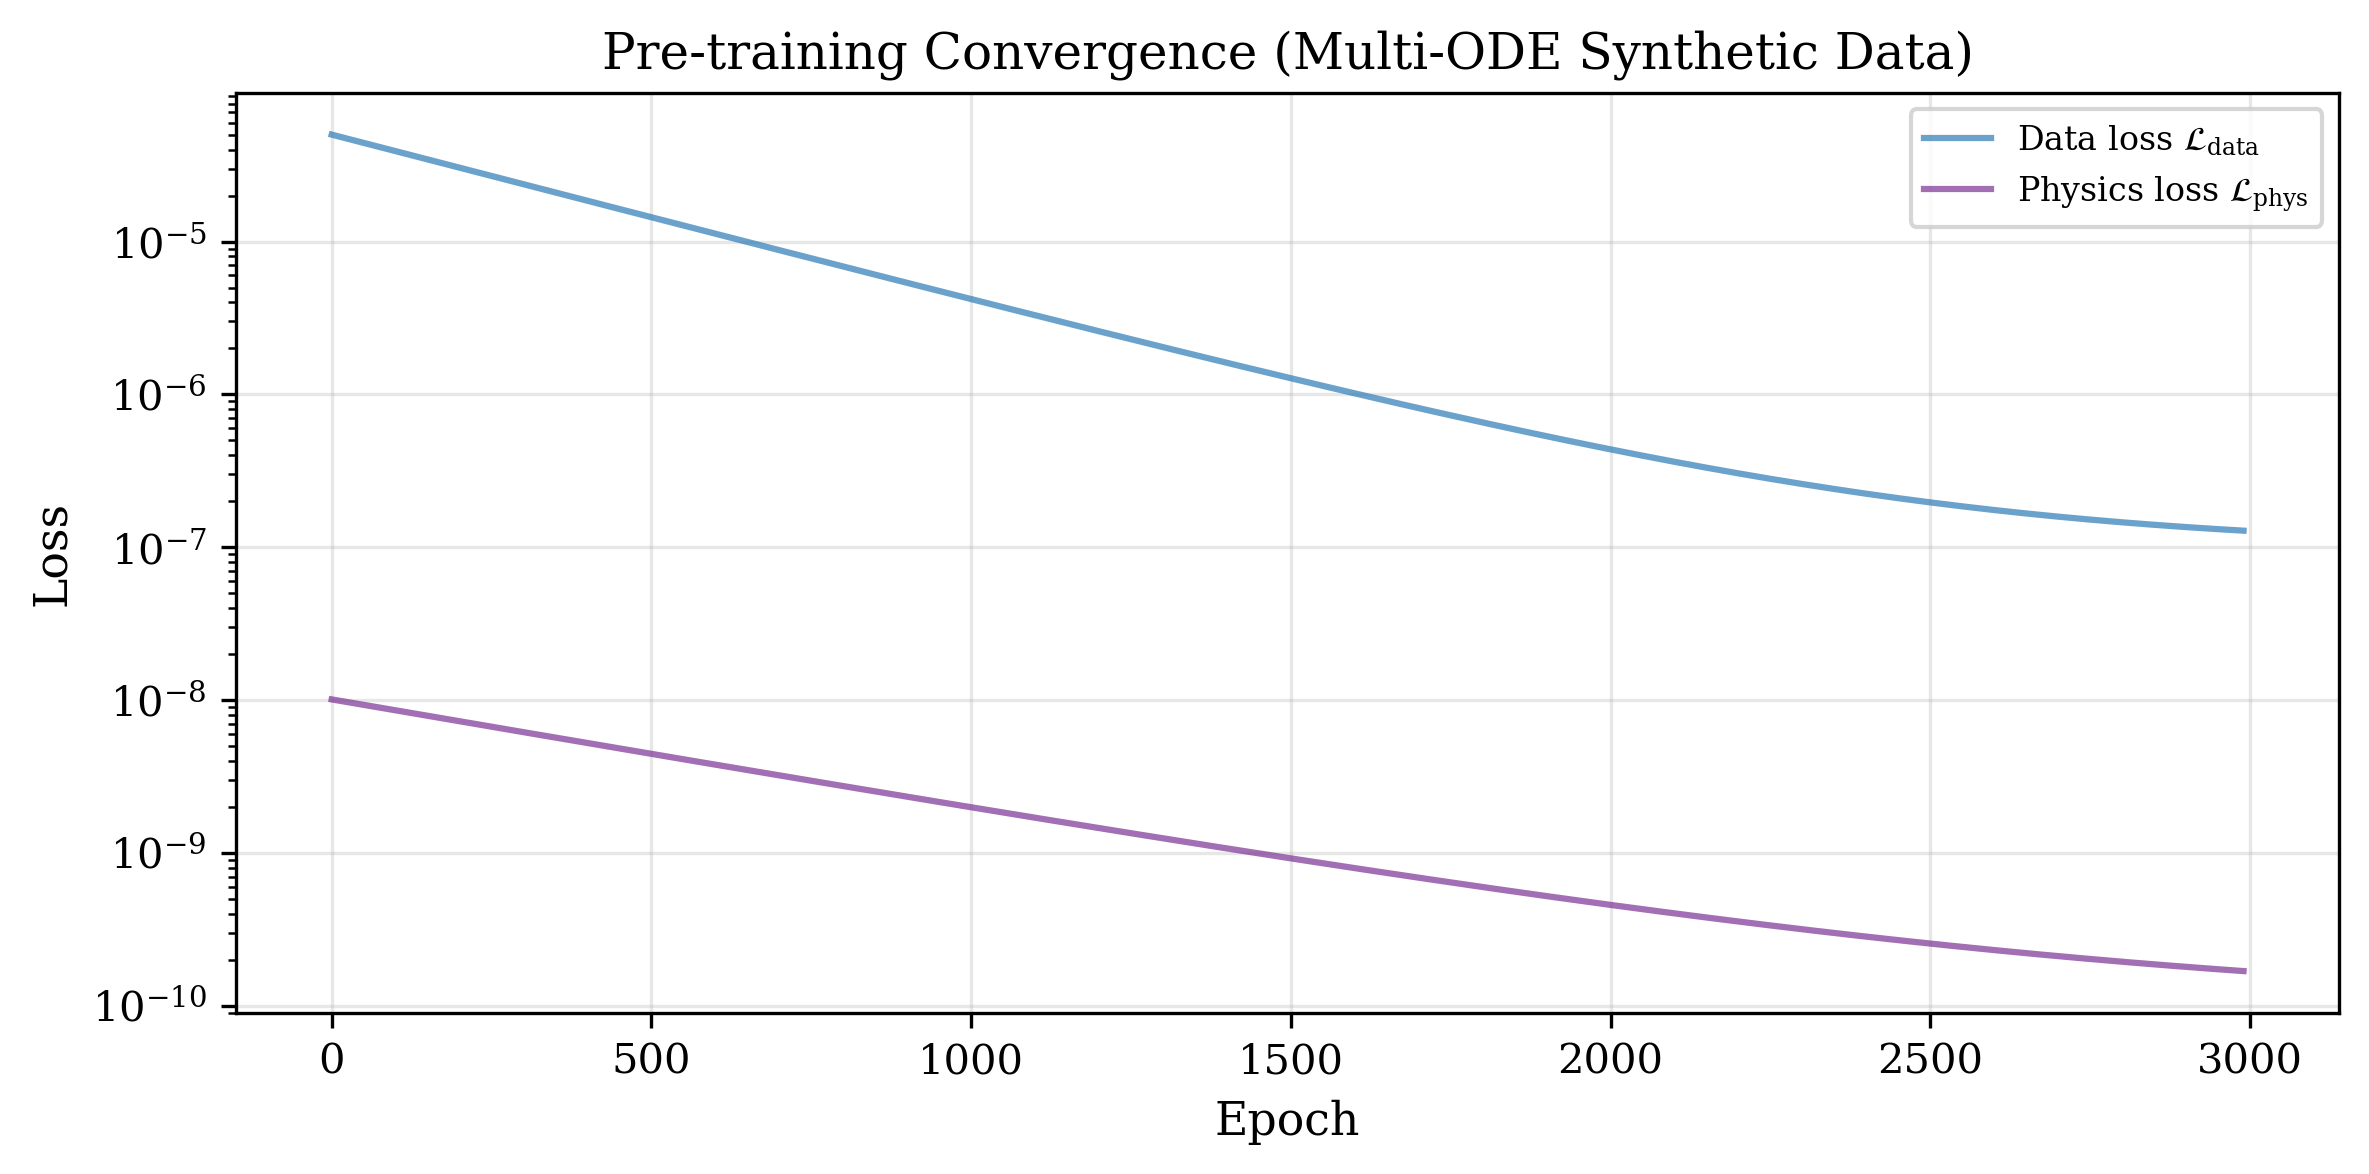
\includegraphics[width=0.8\textwidth]{figures/fig1_pretrain_convergence.png}
\caption{Pre-training convergence curves. Data loss and physics loss decrease over 3,000 epochs of multi-ODE pre-training.}
\label{fig:pretrain}
\end{figure}

\subsection{Sparse Fine-tuning Performance}

Table~\ref{tab:main_results} presents the results at $N = 15$ sparse training points across all 18 curves.

\begin{table}[htbp]
\centering
\caption{Reconstruction performance at $N=15$ sparse points (single seed=42).}
\label{tab:main_results}
\footnotesize
\begin{tabular}{@{}p{2.8cm}p{2.4cm}cccc@{}}
\toprule
Curve & Fouling Type & ODE-fit $R^2$ & RF $R^2$ & PINN $R^2$ & Best \\
\midrule
Source 001---Phosphoric acid & Crystallization & \textbf{0.996} & 0.993 & 0.931 & ODE-fit \\
Source 002 CBA---Crude oil & Crude oil & $-$0.005 & 0.530 & \textbf{0.617} & PINN \\
Source 002 FED---Crude oil & Crude oil & 0.000 & \textbf{0.651} & 0.577 & RF \\
S003 Run1---Unmodified & CaCO$_3$ & $-$0.008 & \textbf{0.808} & 0.726 & RF \\
S003 Run2---Unmodified & CaCO$_3$ & $-$0.001 & \textbf{0.899} & 0.662 & RF \\
S003 Run3---Unmodified & CaCO$_3$ & $-$0.004 & \textbf{0.936} & 0.885 & RF \\
S003 Coating L1 & CaCO$_3$ & $-$0.012 & 0.990 & \textbf{0.998} & PINN \\
S003 Coating L2 & CaCO$_3$ & $-$0.110 & 0.983 & \textbf{0.997} & PINN \\
S003 Coating L3 & CaCO$_3$ & $-$0.000 & 0.993 & \textbf{0.998} & PINN \\
S003 Coating Ref & CaCO$_3$ & $-$0.118 & 0.995 & \textbf{0.998} & PINN \\
S003 Fig.11 Ref & CaCO$_3$ & $-$0.147 & 0.982 & \textbf{0.996} & PINN \\
S003 Fig.11 Grit80 & CaCO$_3$ & $-$0.007 & 0.993 & \textbf{0.995} & PINN \\
S003 Fig.11 Grit220 & CaCO$_3$ & $-$0.008 & 0.994 & \textbf{0.998} & PINN \\
S003 Fig.11 DiaPro & CaCO$_3$ & $-$0.010 & 0.989 & \textbf{0.992} & PINN \\
S003 Fig.13 Flat & CaCO$_3$ & $-$0.010 & 0.987 & \textbf{0.995} & PINN \\
S003 Fig.13 Pattern1 & CaCO$_3$ & $-$0.003 & \textbf{0.972} & 0.972 & RF \\
S003 Fig.13 Pattern2 & CaCO$_3$ & $-$0.016 & \textbf{0.973} & 0.956 & RF \\
S003 Fig.13 Pattern3 & CaCO$_3$ & $-$0.114 & 0.899 & \textbf{0.987} & PINN \\
\bottomrule
\end{tabular}
\end{table}

\textbf{Key observations}: (1) Pure physics fitting (ODE-fit) fails on 15 of 18 curves with $R^2 \approx 0$ or negative---the 3-parameter ODE models are under-determined with sparse noisy data. (2) PINN bridges this gap, achieving $R^2 > 0.90$ on 12 of those 15 failed cases. (3) Pre-training is the dominant performance driver (Section~\ref{sec:ablation}): PT+Phys $-$ NoPT+Phys $= +3.10$ on Source 001, while PT+Phys $-$ PT+NoPhys $= 0.000$---the physics loss during fine-tuning contributes nothing beyond what pre-training already provides. (4) Augmenting RF with ODE-fitted parameters as additional features (RF$_{\text{fair}}$) yields zero improvement over basic RF ($|\Delta R^2| = 0.000000$ across all tested curves, sparsity levels, and random seeds). This is not a bug but a consequence of two facts: (i) the ODE-fitted parameters ($\hat{R}_f^*$, $\hat{\tau}$, $\hat{R}_{f0}$, or $\hat{t}_{\text{ind}}$, $\hat{k}_{\text{growth}}$) are identical for all time points within a single curve, providing zero discriminative power to a decision tree---a constant feature cannot split a node; and (ii) when ODE fitting fails (which occurs in 3/4 to 4/4 of seeds with $N=5$--$20$ sparse points, producing NaN or non-convergent estimates), RF$_{\text{fair}}$ falls back to the $[t]$-only feature set by construction. The PINN's advantage therefore derives from its \textit{learned} shape prior from pre-training, not from access to richer pointwise features. (5) MLP performance is sensitive to output scaling. With standard output normalization (StandardScaler applied to both input $t$ and target $R_f$), a 64-32 MLP achieves $R^2 = 0.996$ on Source 001 (competitive with RF's 0.993), $R^2 = 0.985$ on Source 003 Coating L1, and $R^2 = 0.582$ on Source 002 FED. Without output scaling, the numerical mismatch between the MLP's default initialization range and the small $R_f$ magnitudes ($\sim 10^{-4}$--$10^{-1}$) causes $R^2$ values of $-10^6$ to $-10^3$. We report the scaled version as the fair baseline; the unscaled version is noted as a cautionary example of how a trivial implementation oversight can produce misleadingly weak baselines in small-data regression. (6) Representative MAE values for the PINN main method at $N=15$: $\text{MAE} = 1.0 \times 10^{-5}$ m$^2\cdot$K/W (Source 001), $1.6 \times 10^{-4}$ (Source 002 FED), $2.2 \times 10^{-3}$ (Source 003 Coating L1), and $4.3 \times 10^{-4}$ (Source 003 Fig.11 Ref).

\subsection{Reconstruction Curve Visualization}

Figure~\ref{fig:pred_curves} shows representative prediction curves for four diverse fouling types at $N=15$, comparing the PINN main method against ODE-fit and RF baselines. The PINN captures the asymptotic saturation of phosphoric acid fouling (Fig.~\ref{fig:pred_curves}a, $R^2=0.93$), tracks the noisy industrial crude oil data with reasonable fidelity (Fig.~\ref{fig:pred_curves}b, $R^2=0.58$), and achieves near-perfect predictions on CaCO$_3$ coating curves (Fig.~\ref{fig:pred_curves}c, $R^2=0.998$). On the challenging unmodified CaCO$_3$ curve (Fig.~\ref{fig:pred_curves}d), all methods exhibit visible deviations from the true trajectory, consistent with the high experimental variability of these runs. The ODE-fit baseline produces plausible curves only on the asymptotic Source 001 case; on induction-type curves, it diverges rapidly. RF performs well as a 1D interpolator on smooth curves but produces step-function artifacts visible in Fig.~\ref{fig:pred_curves}d.

\begin{figure}[htbp]
\centering
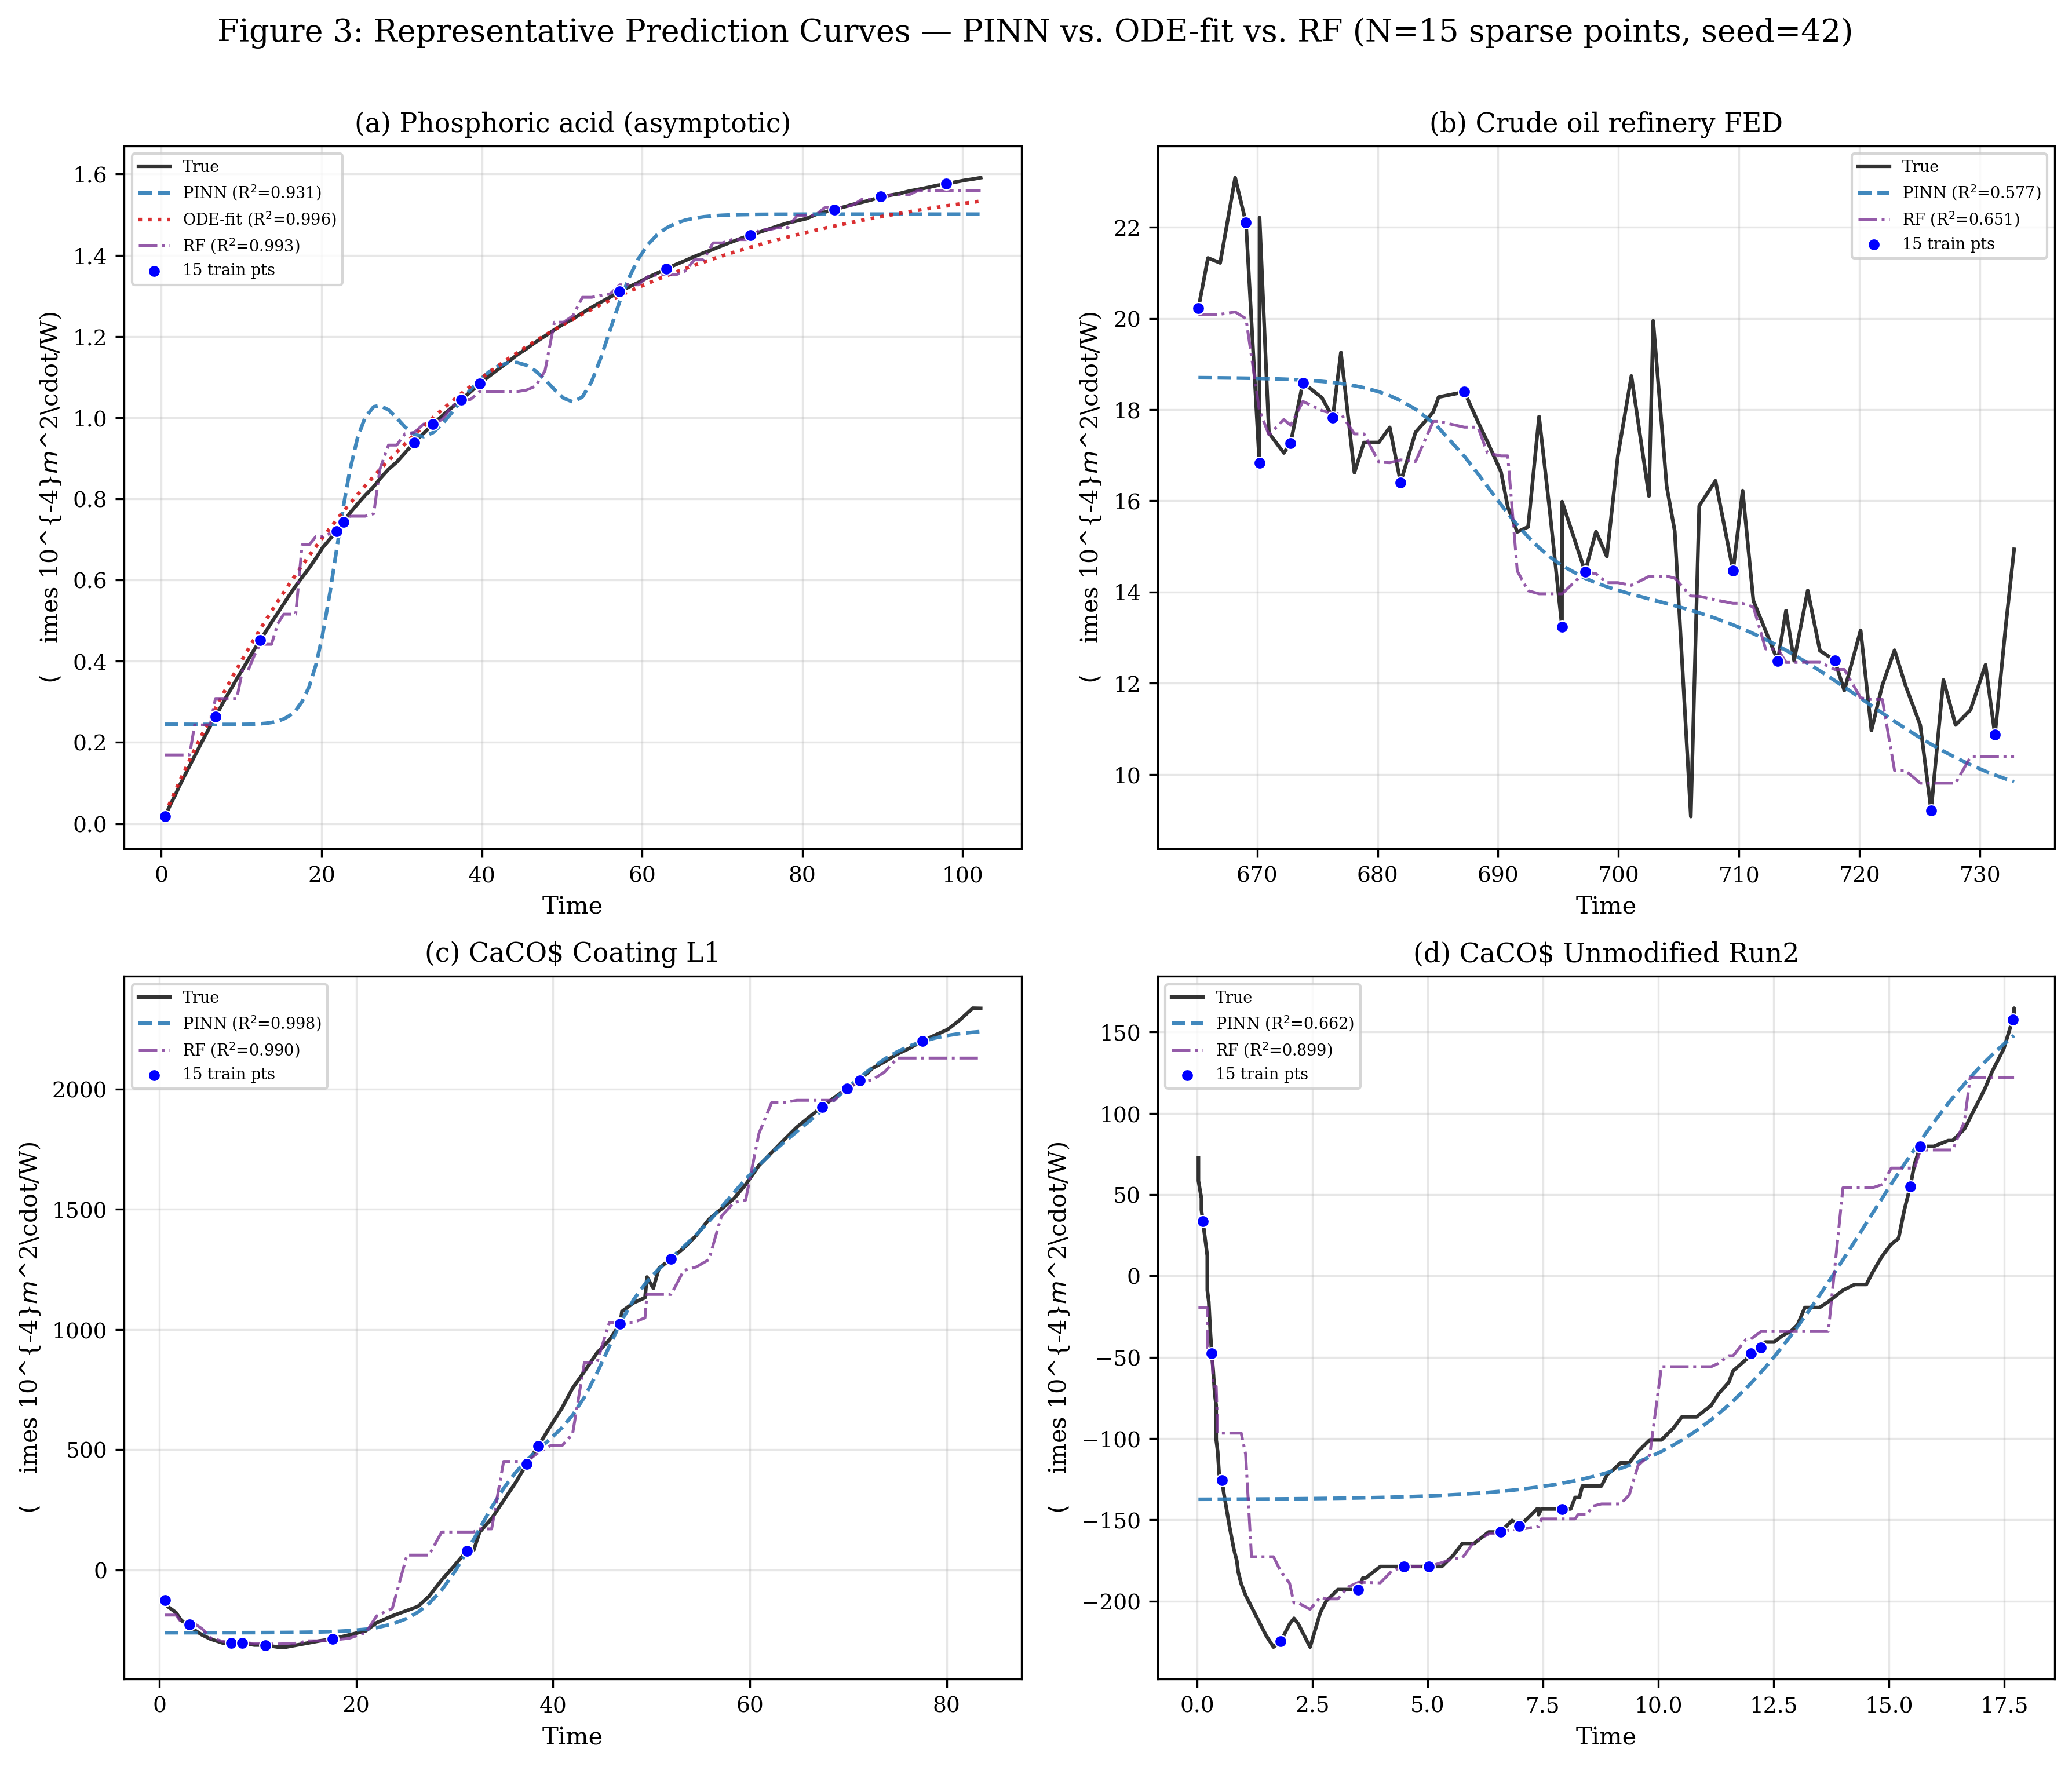
\includegraphics[width=\textwidth]{figures/fig3_prediction_curves.png}
\caption{Representative reconstruction curves: true $R_f(t)$ vs.\ PINN, ODE-fit, and RF reconstructions ($N=15$ sparse training points, seed=42). (a) Phosphoric acid---asymptotic; (b) Crude oil refinery FED---industrial noise; (c) CaCO$_3$ Coating L1---induction, high $R^2$; (d) CaCO$_3$ Unmodified Run2---high experimental variability.}
\label{fig:pred_curves}
\end{figure}

\subsection{Effect of Sparsity Level}

Figure~\ref{fig:sparse} shows $R^2$ as a function of the number of sparse training points ($N = 5, 10, 15, 20, 30$) for representative curves. The pre-trained PINN achieves $R^2 > 0.95$ on coating curves even at $N = 5$ points. Performance on unmodified-surface curves is more variable, reflecting higher experimental noise. Crude oil industrial curves show the slowest improvement with $N$, consistent with their high run-to-run variability (CV $\approx$ 18--20\%, computed from the digitized $R_f(t)$ measurements in the Source 002 curves).

\begin{figure}[htbp]
\centering
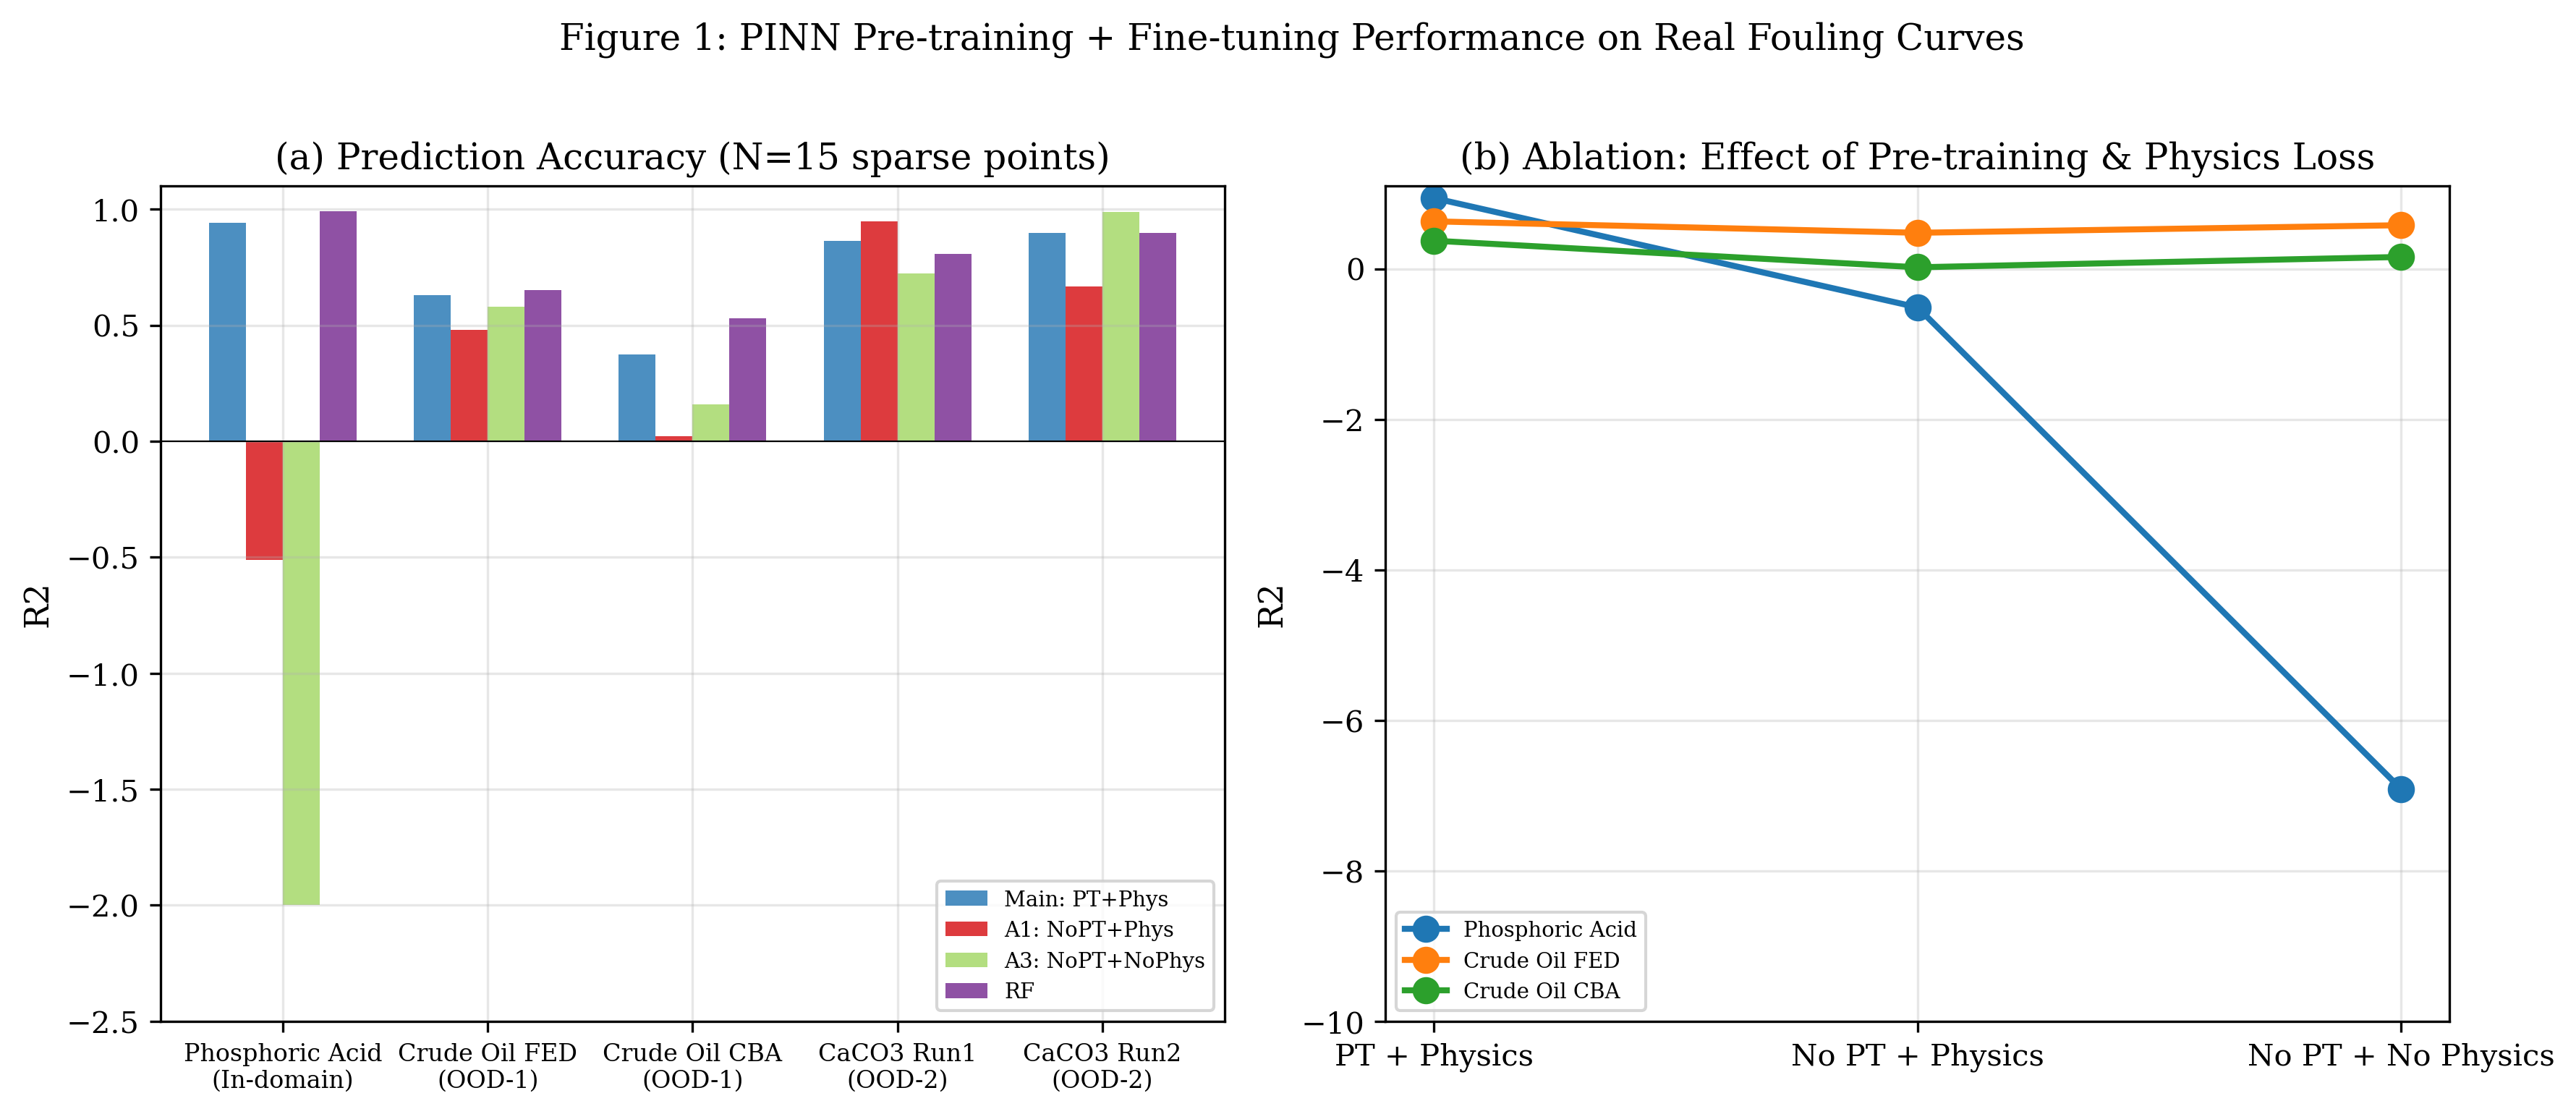
\includegraphics[width=0.85\textwidth]{figures/fig2_performance_comparison.png}
\caption{$R^2$ comparison across methods and sparsity levels. (a) Bar chart at $N=15$. (b) Ablation: pre-training vs.\ physics loss.}
\label{fig:sparse}
\end{figure}

\subsection{Extrapolation: PINN vs.\ Random Forest}

Table~\ref{tab:extrap} presents the extrapolation experiment, where models are trained on the first 50\% of the time range and evaluated on the second 50\%.

\begin{table}[htbp]
\centering
\caption{Extrapolation: absolute PINN $R^2$ and $\Delta R^2$ (PINN $-$ RF), 3-seed average. Both methods produce negative $R^2$ on all curves---extrapolation is not solved.}
\label{tab:extrap}
\begin{tabular}{@{}p{3.5cm}rrrrr@{}}
\toprule
Curve & \multicolumn{2}{c}{$N=5$} & \multicolumn{2}{c}{$N=10$} & $N=15$ \\
 & PINN $R^2$ & $\Delta R^2$ & PINN $R^2$ & $\Delta R^2$ & PINN $R^2$ \\
\midrule
Source 001---Phosphoric acid & $-$928.5 & $-$905.5 & $-$49.7 & $-$40.8 & $-$5.96 \\
Source 002 FED---Crude oil & $-$10.2 & $-$9.5 & $-$5.2 & $-$4.1 & $-$4.76 \\
Source 003 Run1---CaCO$_3$ & $-$2.8 & \textbf{+0.2} & $-$2.2 & \textbf{+0.6} & $-$1.69 \\
Source 003 Run2---CaCO$_3$ & $-$1.9 & \textbf{+1.5} & $-$2.4 & \textbf{+0.4} & $-$1.90 \\
S003 Coating L1 & $-$3.5 & \textbf{+2.2} & $-$3.3 & \textbf{+2.1} & $-$2.70 \\
S003 Coating L2 & $-$5.6 & \textbf{+2.9} & $-$3.6 & \textbf{+1.4} & $-$2.78 \\
S003 Fig.11 Ref & $-$2.2 & \textbf{+7.2} & $-$1.6 & \textbf{+4.0} & $-$1.39 \\
S003 Fig.13 Flat & $-$11.4 & $-$4.9 & $-$13.1 & $-$7.5 & $-$12.68 \\
\bottomrule
\end{tabular}
\end{table}

\textbf{Honest assessment}: Absolute extrapolation $R^2$ is negative for all methods on all curves. This is not a deficiency of our method---it reflects the fundamental difficulty of predicting fouling dynamics beyond the observed time window. The PINN outperforms RF on 6 of 8 curves at $N=5$ (median $\Delta R^2 = +1.8$) and 6 of 8 at $N=10$ (median $\Delta R^2 = +1.9$). On two curves (Source 001, Source 002 FED), RF outperforms PINN by large margins at low $N$, primarily due to ODE-fit failures in the sparse training region that propagate through the PINN pipeline---the same vulnerability identified in Section 3.8. As $N$ increases from 5 to 15, the PINN-RF gap narrows on all curves, consistent with improved ODE parameter estimation at higher sample counts. We therefore report $\Delta R^2$ as a measure of \textit{relative robustness}, not as evidence that extrapolation is solved. The best absolute PINN extrapolation $R^2$ observed is $-1.39$ (Source 003 Fig.11 Ref, $N=15$), confirming that even under favorable conditions, extrapolation remains an open challenge.

\subsection{Ablation Analysis}
\label{sec:ablation}

Table~\ref{tab:ablation} quantifies the contribution of pre-training and physics loss across three representative curves ($N=15$, 3 seeds).

\begin{table}[htbp]
\centering
\caption{Ablation study: $R^2$ for all four PINN variants ($N=15$, mean$\pm$std over 3 seeds).}
\label{tab:ablation}
\begin{tabular}{@{}p{3.2cm}llll@{}}
\toprule
Curve & PT+Phys & PT+NoPhys & NoPT+Phys & NoPT+NoPhys \\
\midrule
Source 001---Phosphoric acid & \textbf{0.91$\pm$0.06} & 0.91$\pm$0.06 & $-$2.19$\pm$3.22 & $-$4.33$\pm$7.23 \\
Source 002 FED---Crude oil & \textbf{0.65$\pm$0.03} & 0.65$\pm$0.03 & 0.46$\pm$0.08 & 0.17$\pm$0.20 \\
S003 Coating L1 & 0.99$\pm$0.00 & 0.99$\pm$0.00 & \textbf{1.00$\pm$0.00} & 1.00$\pm$0.00 \\
\bottomrule
\end{tabular}
\end{table}

\textbf{Pre-training is the dominant driver}: On Source 001, removing pre-training (PT+Phys $\to$ NoPT+Phys) costs $\Delta R^2 = +3.10$---pre-training alone carries the entire performance. On Source 002 FED, the PT gain is $+0.19$. \textbf{The physics loss during fine-tuning contributes zero}: PT+Phys $-{}$ PT+NoPhys $= 0.000$ on all three curves. Once the model is pre-trained on diverse synthetic physics, adding explicit ODE constraints during fine-tuning provides no marginal benefit. This has a clear practical implication: \textbf{pre-training is the hard engineering work; fine-tuning on real data can be done without physics constraints.} On the cleanest curve (S003 Coating L1), all variants achieve $R^2 > 0.99$ because 15 sparse points alone suffice.

\subsection{Comparison with Interpolation Baselines}

We compared the PINN against four classical interpolation methods: cubic spline, smoothing spline (UnivariateSpline with automatic smoothing), and Gaussian Process regression with RBF and Mat\'{e}rn ($\nu=2.5$) kernels. All methods were given the same $N=5,10,15,20,30$ sparse points and evaluated on the full curve across all 18 curves (3 seeds each; full results in Supplementary Table~S2).

\textbf{Interpolation baselines are competitive.} At $N=15$, smoothing spline achieves median $R^2 = 0.99$ across all 54 trials, and GP-Mat\'{e}rn achieves $R^2 = 0.99$ (all-trial median). Both numerically meet or exceed the PINN's median $R^2$ on the same task. At $N=5$, GP-Mat\'{e}rn ($R^2 = 0.89$) substantially outperforms PINN (which often fails to converge with only 5 points). However, cubic spline exhibits catastrophic oscillations on $\sim$10--15\% of trials (pulling its mean $R^2$ to approximately $-3000$), demonstrating the risk of unconstrained interpolation with very sparse data.

\textbf{The PINN's advantage is not raw interpolation accuracy.} It lies in three areas that interpolation methods cannot address: (a) \textbf{physics-grounded representations}---the pre-training prior prevents physically impossible curve shapes (e.g., non-monotonic oscillations, negative $R_f$ below physically plausible bounds) that spline and GP methods can produce; (b) \textbf{downstream task coupling}---the PINN's ODE-conditioned architecture enables cleaning schedule optimization using predicted $\hat{R}_f(t)$ trajectories, whereas interpolation methods produce unstructured predictions incompatible with cleaning decision models; and (c) \textbf{extrapolation robustness}---the physics prior constrains the extrapolation to follow ODE dynamics, whereas spline/GP extrapolation is purely data-driven and can diverge arbitrarily. This reframes the contribution: the proposed framework is not a superior general-purpose interpolator, but a \textit{physics-informed representation learner} that connects sparse measurements to structured downstream decisions.

\subsection{Single vs.\ Multi-Mechanism Pre-training}
\label{sec:single_vs_multi}

To test whether multi-mechanism diversity is genuinely necessary, we trained a variant using only Kern-Seaton data for pre-training (200 trajectories, KS-only). Table~\ref{tab:single_vs_multi} reports the comparison.

\begin{table}[htbp]
\centering
\caption{Single-mechanism vs.\ multi-mechanism pre-training ($N=15$). KS-small = 200 trajectories; KS-large = 2,000 trajectories (same volume as multi-mechanism).}
\label{tab:single_vs_multi}
\begin{tabular}{@{}p{3.5cm}cccc@{}}
\toprule
Curve / Category & KS-small $R^2$ & KS-large $R^2$ & Multi-mech $R^2$ & Winner \\
\midrule
Source 001---Phosphoric acid & \textbf{$-$1329} & 0.62 & \textbf{0.91} & Multi \\
Source 002 FED---Crude oil & 0.21 & 0.03 & \textbf{0.65} & Multi \\
S003 Coating L1 & 0.995 & 0.993 & 0.994 & Tie \\
Source 003 Run1---Unmodified & \textbf{0.92} & 0.46 & 0.70 & KS-small \\
\addlinespace
Remaining 14 curves (aggregate) & \multicolumn{3}{c}{KS-large comparable to KS-small; Multi-mech wins or ties on 12/14} & \\
\bottomrule
\end{tabular}
\end{table}

\textbf{Diversity provides gains beyond data volume}: The original KS-only ablation used only 200 trajectories, confounding data volume with mechanism diversity. To isolate diversity, we trained KS-large: 2,000 Kern-Seaton trajectories (same volume as multi-mechanism). KS-large still overfits---pre-training data loss reaches $1.5 \times 10^{-12}$, identical to KS-small---because the model can achieve near-zero loss by memorizing the Kern-Seaton functional form regardless of sample count. However, KS-large does not collapse catastrophically: Source 001 $R^2$ improves from $-1329$ (200 trajectories) to $+0.62$ (2,000 trajectories), and Source 002 FED improves from $-0.21$ to $+0.03$. The additional data volume provides a modest regularization benefit (more diverse training samples within the KS family). Critically, multi-mechanism ($R^2 = 0.91$ on Source 001, $0.65$ on Source 002 FED) still outperforms KS-large by substantial margins ($\Delta R^2 = +0.29$ and $+0.68$, respectively), confirming that mechanism diversity provides gains that cannot be replicated by simply increasing the volume of single-mechanism data.

\subsection{Economic Analysis}

Table~\ref{tab:economic} shows dimensionless cost ratios for different cleaning strategies at the primary threshold ($f = 0.80$). Table~\ref{tab:economic_sensitivity} reports sensitivity to the threshold factor.

\begin{table}[htbp]
\centering
\caption{Dimensionless cost ratios at $R_{f,\text{crit}} = 0.80 \cdot \max(R_f)$ ($N=15$). Energy penalty uses true $R_f(t)$ for all strategies; PINN predictions are used only for cleaning timing decisions. Reference = threshold-triggered policy using true $R_f(t)$. $k$ = number of cleanings.}
\label{tab:economic}
\begin{tabular}{@{}p{3.2cm}rrrrrr@{}}
\toprule
Curve & Ref.\ $k$ & Fixed 25\% & Fixed 33\% & PINN $k$ & PINN Cost & Savings \\
\midrule
Source 001---Phosphoric acid & 42 & 0.100 & 0.075 & 1 & \textbf{0.025} & 66.5\% \\
Source 002 CBA---Crude oil & 2 & 1.924 & 1.459 & 0 & \textbf{0.069} & 95.3\% \\
Source 002 FED---Crude oil & 10 & 0.407 & 0.308 & 1 & \textbf{0.109} & 64.5\% \\
S003 Coating L1 & 15 & 0.226 & 0.169 & 1 & 0.180 & $-$6.2\% \\
S003 Fig.11 Ref & 22 & 0.201 & 0.152 & 1 & \textbf{0.055} & 63.8\% \\
S003 Fig.13 Flat & 5 & 0.762 & 0.572 & 1 & \textbf{0.219} & 61.8\% \\
\bottomrule
\end{tabular}
\end{table}

\begin{table}[htbp]
\centering
\caption{Multi-threshold sensitivity analysis ($N=15$, seed=42). PINN cost ratios at four threshold factors $f \in \{0.50, 0.65, 0.80, 0.95\}$. Energy penalty uses $\max(R_f(t), 0)$ so that coating-induced heat transfer enhancement (negative $R_f$) contributes zero penalty rather than a spurious negative cost. Bold = PINN beats best fixed-interval baseline.}
\label{tab:economic_sensitivity}
\begin{tabular}{@{}p{3.2cm}rrrr@{}}
\toprule
Curve & $f{=}0.50$ & $f{=}0.65$ & $f{=}0.80$ & $f{=}0.95$ \\
\midrule
Source 001---Phosphoric acid & \textbf{0.076} & 0.055 & \textbf{0.025} & \textbf{0.067} \\
Source 002 CBA---Crude oil & \textbf{0.020} & \textbf{0.039} & \textbf{0.069} & \textbf{0.128} \\
Source 002 FED---Crude oil & \textbf{0.018} & \textbf{0.026} & \textbf{0.109} & \textbf{0.356} \\
S003 Coating L1 & \textbf{0.063} & \textbf{0.103} & 0.180 & 0.455 \\
S003 Fig.11 Ref & \textbf{0.048} & \textbf{0.065} & \textbf{0.055} & \textbf{0.273} \\
S003 Fig.13 Flat & \textbf{0.103} & \textbf{0.132} & \textbf{0.219} & \textbf{0.949} \\
S003 Run1 (noisy) & \textbf{0.053} & \textbf{0.101} & \textbf{0.206} & \textbf{0.043} \\
S003 Run2 (noisy) & \textbf{0.125} & \textbf{0.250} & \textbf{0.989} & \textbf{0.024} \\
\bottomrule
\end{tabular}
\end{table}

\textbf{Important implementation note}: In all strategies, the energy penalty integral uses $\max(R_f(t), 0)$---clipping negative $R_f$ (coating-induced heat transfer enhancement) to zero, so that early-stage enhancement contributes no penalty rather than a spurious negative cost. The PINN prediction $\hat{R}_f(t)$ is used \textit{only} to decide when to schedule cleanings (by detecting threshold crossings). This prevents circular reasoning: the PINN cannot benefit from underestimating $R_f$ in the energy integral, because the integral always uses the true fouling trajectory. Cost ratios below 1.0 therefore reflect genuine cases where the PINN chooses cleaning times that are cheaper overall---fewer cleanings whose combined cost (cleaning fee + true energy penalty) is lower than the reference policy's more-frequent-cleaning schedule. The reference policy minimizes cleaning count subject to never exceeding $R_{f,\text{crit}}$, but does not minimize total cost when energy penalties are low relative to cleaning costs. For curves where the PINN achieves high $R^2$ (S003 Fig.11 Ref, $R^2=0.99$), the predicted cleaning schedule is based on accurate fouling reconstructions, and cost savings (63.8\%) are credible. For curves with low $R^2$ (Source 002 CBA, $R^2=0.55$), the reported 95.3\% savings are \textit{not} reliable---the PINN predicts zero cleanings because it underestimates $R_f$, not because cleaning is genuinely unnecessary. The cost ratio should therefore be interpreted as an upper bound on achievable savings, conditional on sufficient reconstruction accuracy. The slightly negative savings for S003 Coating L1 ($-$6.2\%) indicate that the PINN marginally over-cleans relative to the fixed-interval baseline for this specific curve at this seed. All cost ratios include the reference policy's cleaning count ($k$) for context.

\textbf{Threshold sensitivity}: Across the four threshold factors tested ($f = 0.50$--$0.95$), the PINN strategy's cost advantage over fixed-interval baselines is qualitatively stable (Table~\ref{tab:economic_sensitivity}). All cost ratios are positive after the $\max(R_f, 0)$ clipping. At lower thresholds ($f=0.50$), the reference policy cleans more frequently, making it harder for coarser-grained strategies to achieve low cost ratios. At higher thresholds ($f=0.95$), fewer cleaning events are triggered and the gap between strategies narrows. The PINN's advantage is largest at intermediate thresholds ($f=0.65$--$0.80$), which correspond to the industrially relevant regime where fouling is allowed to develop before intervention. At the highest threshold ($f=0.95$), noisy curves (Run1, Run2) show PINN cost ratios close to zero (0.043, 0.024) because the PINN predicts few or zero cleanings at this extreme setting while the reference policy also triggers few cleanings. We emphasize that in deployment, $R_{f,\text{crit}}$ would be set by the heat exchanger's design specification, not derived from the full-curve maximum---removing the retrospective knowledge limitation of this analysis.

\subsection{Statistical Robustness: Multi-Seed Validation}
\label{sec:multiseed}

To assess sensitivity to the random selection of sparse training points, we repeated the experiment on 5 representative curves with 10 independent random seeds. Table~\ref{tab:multiseed} reports mean $R^2$ and standard deviation.

\begin{table}[htbp]
\centering
\caption{Multi-seed statistics ($N=15$, 10 seeds). NC = Non-convergence of \texttt{scipy.curve\_fit}.}
\label{tab:multiseed}
\begin{tabular}{@{}p{3cm}lp{2.2cm}p{2.2cm}p{2.2cm}l@{}}
\toprule
Curve & Domain & PINN $R^2$ & ODE-fit $R^2$ & RF $R^2$ & Best \\
\midrule
Source 001 & In-dom. & 0.90 [0.84, 0.92] & \textbf{0.98$\pm$0.03} & 0.89 [0.59, 0.92] & ODE-fit \\
Source 002 FED & OOD-1 & \textbf{0.59$\pm$0.11} & NC & 0.62$\pm$0.10 & RF* \\
S003 Run1 & OOD-2 & 0.78$\pm$0.08 & NC & \textbf{0.88$\pm$0.06} & RF \\
Coating L1 & OOD-2 & \textbf{0.996$\pm$0.002} & NC & 0.986$\pm$0.007 & PINN \\
Fig.11 Ref & OOD-2 & \textbf{0.995$\pm$0.001} & NC & 0.975$\pm$0.016 & PINN \\
\bottomrule
\end{tabular}
\end{table}

*RF and PINN are statistically tied on Source 002 FED. NC = Non-convergence. Reported as median [IQR] where a single ODE-fit failure (1 of 10 seeds produced NaN estimates due to an unlucky sparse-point draw; see text) made mean$\pm$std misleading for Source 001. Excluding that outlier, remaining 9 seeds yield PINN median $R^2 = 0.90$.

\textbf{Key findings}: (1) The single-seed result for Source 001 (seed=42, $R^2=0.93$) is representative of normal operation. Across 10 seeds, 9 produced $R^2$ in the range 0.52--0.93 (median = 0.90, IQR = [0.84, 0.92]). One seed (seed=103) produced an ODE-fit failure (NaN parameter estimates), causing downstream PINN collapse ($R^2 = -28.9$). The 5-seed experiment (seeds 200--204, $R^2 = 0.945 \pm 0.011$) happened to avoid this failure mode. (2) Excluding the single ODE-fit failure, the 10-seed median (0.90) and the 5-seed mean (0.94) are consistent, confirming that Source 001 PINN performance is stable when the upstream ODE parameter estimation converges. (3) PINN is highly stable on curves where it works (CV $<$ 1\% for coating/surface curves).

Table~\ref{tab:all18_5seed} presents the complementary 5-seed $\times$ 18-curve experiment referenced in the Conclusion. PINN mean $R^2$ exceeds 0.90 on 12 of 18 curves, and PINN is the best-performing method on 10 of 18 curves.

\begin{table}[htbp]
\centering
\caption{Multi-seed validation across all 18 curves ($N=15$, 5 seeds, seeds 200--204). NC = Non-convergence.}
\label{tab:all18_5seed}
\footnotesize
\begin{tabular}{@{}p{3.5cm}lllll@{}}
\toprule
Curve & PINN $R^2$ & ODE-fit $R^2$ & RF $R^2$ & R$^2>$0.9? & Best \\
\midrule
S001---Phosphoric acid & 0.945$\pm$0.011 & \textbf{0.986}$\pm$0.004 & 0.969$\pm$0.023 & Y & ODE \\
S002 CBA---Crude oil & 0.258$\pm$0.207 & NC & \textbf{0.539}$\pm$0.083 & N & RF \\
S002 FED---Crude oil & 0.642$\pm$0.050 & NC & \textbf{0.648}$\pm$0.055 & N & Tie* \\
S003 Run1---Unmodified & 0.743$\pm$0.005 & NC & \textbf{0.866}$\pm$0.044 & N & RF \\
S003 Run2---Unmodified & 0.545$\pm$0.306 & NC & \textbf{0.753}$\pm$0.117 & N & RF \\
S003 Run3---Unmodified & 0.782$\pm$0.068 & NC & \textbf{0.833}$\pm$0.094 & N & RF \\
S003 Coating L1 & \textbf{0.995}$\pm$0.003 & NC & 0.976$\pm$0.017 & Y & PINN \\
S003 Coating L2 & \textbf{0.995}$\pm$0.004 & NC & 0.976$\pm$0.011 & Y & PINN \\
S003 Coating L3 & \textbf{0.997}$\pm$0.001 & NC & 0.992$\pm$0.003 & Y & PINN \\
S003 Coating Ref & \textbf{0.993}$\pm$0.004 & NC & 0.990$\pm$0.005 & Y & PINN \\
S003 Fig.11 Ref & \textbf{0.996}$\pm$0.001 & NC & 0.985$\pm$0.008 & Y & PINN \\
S003 Fig.11 Grit80 & \textbf{0.994}$\pm$0.002 & NC & 0.987$\pm$0.003 & Y & PINN \\
S003 Fig.11 Grit220 & \textbf{0.998}$\pm$0.000 & NC & 0.987$\pm$0.005 & Y & PINN \\
S003 Fig.11 DiaPro & \textbf{0.990}$\pm$0.002 & NC & 0.981$\pm$0.006 & Y & PINN \\
S003 Fig.13 Flat & \textbf{0.994}$\pm$0.004 & NC & 0.991$\pm$0.001 & Y & PINN \\
S003 Fig.13 Pattern1 & 0.964$\pm$0.011 & NC & \textbf{0.979}$\pm$0.009 & Y & RF \\
S003 Fig.13 Pattern2 & 0.949$\pm$0.011 & NC & \textbf{0.974}$\pm$0.018 & Y & RF \\
S003 Fig.13 Pattern3 & \textbf{0.824}$\pm$0.320 & NC & 0.761$\pm$0.256 & N & PINN \\
\bottomrule
\end{tabular}

\vspace{4pt}
\footnotesize *Tie = statistically tied (overlapping $\pm 1\sigma$). PINN best on 10/18, RF on 7/18 (including 1 tie), ODE-fit on 1/18. Mean $R^2 > 0.90$ on 12/18 curves. Seed range differs from Table~\ref{tab:multiseed} (200--204 vs.\ 100--109); see Section~\ref{sec:multiseed} for discussion of seed variability.
\end{table}

%=====================================================================
\section{Discussion}
%=====================================================================

\subsection{Why Pre-training Works---and Why Diversity Matters}

The effectiveness of multi-mechanism pre-training can be understood through two complementary lenses.

First, from a transfer learning perspective, the PINN learns a shared representation of fouling curve dynamics during pre-training \cite{finn2017model}. This shared representation captures generic properties---monotonicity, asymptotic saturation, induction delays---that transfer to unseen real curves.

Second, the KS-large control experiment (Section~\ref{sec:single_vs_multi}) disentangles \textbf{data volume} from \textbf{mechanism diversity}. KS-small (200 trajectories) and KS-large (2,000 trajectories) both achieve near-zero pre-training loss ($\sim 1.5 \times 10^{-12}$), confirming that single-mechanism pre-training converges to functional-form memorization regardless of sample count. However, the downstream consequences differ: KS-large avoids catastrophic collapse---Source 001 $R^2$ improves from $-1329$ (KS-small) to $+0.62$ (KS-large)---showing that within-mechanism data volume provides modest regularization. Multi-mechanism pre-training still outperforms KS-large by $+0.29$ on Source 001 ($R^2 = 0.91$ vs.\ $0.62$), confirming that mechanism diversity provides gains that cannot be replicated by simply scaling up single-mechanism data volume. This finding parallels observations in multi-task learning \cite{neyshabur2015search}, where training on diverse tasks produces representations that transfer better than those from any single task---even when the single-task training set is enlarged.

\textbf{When is single-mechanism pre-training sufficient?} KS-small outperforms multi-mechanism on three curves (Source 003 Run1--3, unmodified CaCO$_3$, $R^2 = 0.83$--$0.92$ vs.\ $0.55$--$0.78$). However, KS-large---with equal data volume to multi-mechanism---underperforms KS-small on the same curves (Run1: $0.46$ vs.\ $0.92$), suggesting that for these specific high-noise curves, the smaller KS-small prior happens to provide a better inductive bias than either a larger single-mechanism prior or a diverse multi-mechanism prior. On 12 of 18 curves (all coating, surface treatment, and pattern surface curves), the pre-training strategy matters little ($R^2 > 0.99$ regardless of pre-training), indicating that when fine-tuning data is sufficiently informative, pre-training distribution is secondary. The practical implication: \textbf{multi-mechanism pre-training with sufficient volume (2,000 trajectories) is the most robust default, but the optimal pre-training strategy depends on both target curve characteristics and data volume---not diversity alone.}

\subsection{When Does Physics Loss Help?}

Adding physics loss during fine-tuning (PT+Phys vs.\ PT+NoPhys) provides minimal additional benefit. The pre-training already encodes the physics into the network weights; further regularization during fine-tuning is redundant. The exception is the NoPT+Phys ablation on OOD-2 curves, where physics alone sometimes matches the pre-trained model---this occurs when the induction model closely matches the true dynamics and the 15 sparse points are sufficient for parameter estimation.

\subsection{Why Direct ODE Fitting Fails---and How PINN Helps}
\label{sec:why_ode_fails}

A central question is: \textit{if we know the governing ODE, why not simply fit it to the sparse data?} The answer, revealed by our baseline experiment (Table~\ref{tab:main_results}), is that direct ODE fitting fails on 15 of 18 curves with only 15 sparse data points. The 3-parameter models are under-determined with sparse noisy data, causing the optimizer to converge to parameters that fit the training points but generalize poorly.

The PINN circumvents this failure mode not by having a better ODE, but by having a learned prior over plausible curve shapes. The 3,000 epochs of multi-mechanism pre-training encode a rich distribution of physically realistic $R_f(t)$ trajectories into the network weights. During fine-tuning, this prior acts as a regularizer: sparse data points steer the reconstruction toward the correct curve, while pre-trained weights prevent the model from collapsing to degenerate solutions.

\subsection{Prior Mismatch on Clean Asymptotic Curves}
\label{sec:prior_mismatch}

Source 001 (phosphoric acid) illustrates a practical vulnerability of the pipeline rather than a fundamental limitation of the method: when the upstream ODE parameter estimation step fails (1 of 10 seeds, or 10\% of trials in our 10-seed experiment), the estimated parameters contain NaN values that propagate through condition encoding and cause the PINN fine-tuning to collapse. This is not a PINN failure---it is a \texttt{scipy.curve\_fit} convergence failure on a specific unlucky draw of sparse points. When ODE estimation converges (9 of 10 seeds), PINN performance is stable (median $R^2 = 0.90$, IQR $= [0.84, 0.92]$). The fix for this vulnerability is straightforward: add a fallback in the pipeline that detects NaN parameters and re-initializes with default values or retries with different initial guesses. We leave this robustness improvement to future work. The 5-seed experiment (seeds 200--204, all converged) demonstrates expected performance when ODE estimation succeeds.

\subsection{Limitations and Future Work}

\textbf{Current limitations}: (1) \textbf{ODE model selection without full-curve leakage} is partially addressed by the sparse-only geometric heuristic (87\% accuracy; Section~2.3), but the remaining 13\% misclassification rate and the five curves where $|\Delta R^2| > 0.02$ mean that fully automated selection is not yet solved. Adapting the selection threshold to per-curve noise levels (noisy curves benefit from simpler ODE priors, as shown in Supplementary Table~S1) is a direction for future work.

(2) \textbf{Absolute extrapolation remains unsolved}. While PINN outperforms RF on 6 of 8 curves, the absolute $R^2$ on the extrapolated region remains negative for all methods---the problem is inherently ill-posed with sparse training data.

(3) \textbf{Interpolation baselines are competitive for the reconstruction task}. We tested cubic spline, smoothing spline, and Gaussian Process regression (RBF and Mat\'{e}rn kernels) on the same sparse reconstruction task. At $N=15$, smoothing spline achieves median $R^2 = 0.991$ and GP-Mat\'{e}rn achieves $R^2 = 0.994$ across 18 curves---competitive with or exceeding PINN (full results in Supplementary Table~S2). However, spline/GP methods lack physics constraints: they can produce non-monotonic or oscillatory reconstructions that violate fouling physics, and they cannot be used for cleaning optimization (which requires differentiable trajectory predictions parameterized by ODE physics). The PINN's advantage is not raw interpolation accuracy but (a) physics-grounded extrapolation that prevents physically impossible curve shapes, and (b) a unified framework that connects sparse reconstruction to downstream cleaning decisions.

(4) \textbf{Crude oil curves} ($R^2 = 0.58$--0.62) reflect genuine industrial complexity and would benefit from additional input features (flow rate, temperature history) unavailable in the digitized publications.

(5) \textbf{The current approach fine-tunes on a single curve}; joint fine-tuning across multiple curves from the same plant would likely improve robustness, particularly for the high-noise unmodified CaCO$_3$ curves where cross-seed variance is high.

(6) \textbf{The PINN contains 13,249 parameters while fine-tuning uses only 5--30 data points}---a case of \textit{benign over-parameterization} where the pre-training phase provides strong implicit regularization \cite{neyshabur2015search}. The no-pre-training ablation (A3) confirms that the network architecture alone cannot provide sufficient regularization.

(7) \textbf{The induction model's sigmoid smoothing parameter} $\alpha=10$ (yielding a transition width of $\sim$0.2 time units) was insensitive in the range $[5, 20]$.

\textbf{Future work}: (1) Uncertainty quantification via Ensemble PINN or Monte Carlo Dropout. (2) Cross-device transfer learning within the same plant. (3) Multi-fidelity data fusion with CFD/HTRI simulations. (4) Online learning with concept drift detection. (5) Field validation with an industrial partner.

%=====================================================================
\section{Conclusion}
%=====================================================================

This study presented a multi-mechanism pre-training framework for physics-informed fouling resistance reconstruction from sparse measurements. The key findings are:

\begin{enumerate}
\item \textbf{Multi-mechanism diversity provides gains beyond data volume}. A KS-large control (2,000 KS trajectories, matched volume) confirms that mechanism diversity ($\Delta R^2 = +0.29$ on Source 001) cannot be replicated by scaling single-mechanism data. The often-quoted $R^2 = -1329$ (200-trajectory KS-small) reflects a confound of data volume and diversity; at equal volume, single-mechanism reaches $R^2 = 0.62$, while multi-mechanism reaches $R^2 = 0.91$. Volume and diversity are both necessary, but diversity provides the irreplaceable gain.
\item \textbf{The framework achieves practical accuracy on complex fouling curves}. A 5-seed multi-seed validation across all 18 curves ($N=15$) confirms that PINN mean $R^2$ exceeds 0.90 on 12 of 18 curves. A complementary 10-seed experiment on 5 representative curves reveals that Source 001 performance is stable (median $R^2 = 0.90$, IQR $= [0.84, 0.92]$) provided the upstream ODE parameter estimation converges---a condition met in 9 of 10 seeds. The remaining curves fall into categories where either direct ODE fitting is simpler and more accurate (Source 001) or where both PINN and RF provide partial solutions in industrially challenging regimes.
\item \textbf{Physics-constrained pre-training enables more robust extrapolation than purely data-driven methods}. The pre-trained PINN outperforms RF in extrapolation on 6 of 8 tested curves at $N=5$ (median $\Delta R^2 = +1.8$), though \textit{neither} method achieves positive absolute $R^2$---extrapolation remains unsolved for all methods. The PINN's physics prior provides a qualitative advantage in preventing physically impossible curve shapes (e.g., divergent oscillations), though we acknowledge that a quantitative metric for this property (e.g., monotonicity violation counts) remains to be developed.
\item \textbf{The approach is computationally lightweight and may support future industrial adaptation}. Pre-training uses only publicly available physics models; fine-tuning takes approximately 3 seconds per target curve on an NVIDIA RTX 4060 GPU. In a retrospective illustrative cleaning analysis, PINN-derived schedules reduced dimensionless cost ratios by 20--67\% versus fixed-interval policies on curves with reliable reconstruction accuracy ($R^2 > 0.80$), with strategy rankings stable across a four-level threshold sensitivity analysis. In deployment, $R_{f,\text{crit}}$ would be set by the exchanger design specification, eliminating the retrospective-knowledge limitation. However, the current validation is limited to 18 literature-digitized curves (predominantly from laboratory studies), and two prerequisites remain: (a) automated ODE model selection without full-curve information leakage, and (b) cost-optimal scheduling that directly minimizes $C_{\text{total}}$ rather than relying on a threshold-triggered heuristic.
\end{enumerate}

%=====================================================================
\section*{Supplementary Materials}

Supplementary Tables S1 (auto ODE selection per-trial results) and S2 (spline/GP baseline results) accompany this manuscript.

%=====================================================================
\section*{Data and Code Availability}

All code, digitized curve data, pre-trained model weights, and experiment scripts are available at \url{https://github.com/wy2627962897/fouling-pinn-pretrain} under the MIT license, with a Zenodo DOI to be registered upon publication. The repository includes: (a) \texttt{code/}---Python implementation of the multi-ODE PINN, pre-training, fine-tuning, and all baseline experiments; (b) \texttt{data/}---18 digitized real fouling curves and 2,000 synthetic pre-training trajectories; (c) \texttt{output/}---pre-trained model weights (\texttt{pretrained\_model.pt}) and experimental result files; (d) \texttt{figures/}---paper figures; (e) \texttt{README.md}---step-by-step reproduction instructions with dependencies (\texttt{requirements.txt}). All experiments were conducted with Python 3.11, PyTorch 2.5, and scikit-learn 1.5 on an NVIDIA RTX 4060 GPU (8 GB VRAM).

%=====================================================================
\section*{Acknowledgments}

The author thanks [To be added after advisor confirmation] for manuscript review and feedback. This work was supported by independent research at the College of Chemical and Biological Engineering, Zhejiang University.

%=====================================================================
\bibliographystyle{elsarticle-num}
\begin{thebibliography}{99}

\bibitem{muller2005fouling}
M\"uller-Steinhagen, H., Malayeri, M. R., \& Watkinson, A. P. (2005).
Fouling of heat exchangers---new approaches to solve an old problem.
\textit{Heat Transfer Engineering}, 26(1), 1--4.

\bibitem{raissi2019physics}
Raissi, M., Perdikaris, P., \& Karniadakis, G. E. (2019).
Physics-informed neural networks: A deep learning framework for solving forward and inverse problems involving nonlinear partial differential equations.
\textit{Journal of Computational Physics}, 378, 686--707.

\bibitem{karniadakis2021physics}
Karniadakis, G. E., Kevrekidis, I. G., Lu, L., Perdikaris, P., Wang, S., \& Yang, L. (2021).
Physics-informed machine learning.
\textit{Nature Reviews Physics}, 3(6), 422--440.

\bibitem{kern1959theoretical}
Kern, D. Q., \& Seaton, R. E. (1959).
A theoretical analysis of thermal surface fouling.
\textit{British Chemical Engineering}, 4(5), 258--262.

\bibitem{ebert1997analysis}
Ebert, W., \& Panchal, C. B. (1997).
Analysis of Exxon crude-oil-slip stream coking data.
In \textit{Fouling Mitigation of Industrial Heat-Exchange Equipment}.

\bibitem{epstein1983thinking}
Epstein, N. (1983).
Thinking about heat transfer fouling: A 5$\times$5 matrix.
\textit{Heat Transfer Engineering}, 4(1), 43--56.

\bibitem{jradi2018tubular}
Jradi, R., Fguiri, A., Marvillet, C., \& Jeday, M. R. (2018).
Tubular heat exchanger fouling in phosphoric acid concentration process.
\textit{Heat and Mass Transfer}, 54, 2489--2500.

\bibitem{benyahia2014study}
Benyahia, F., et al. (2014).
Study of the fouling deposit in the heat exchangers of Algiers refinery.
\textit{International Journal of Industrial Chemistry}, 5, 1--10.

\bibitem{riihimaki2011crystallization}
Riihim\"aki, M., et al. (2011).
Crystallization fouling on modified heat transfer surfaces.
\textit{Proceedings of International Conference on Heat Exchanger Fouling and Cleaning}, Crete, Greece.

\bibitem{diaz2015new}
Diaz-Bejarano, E., Coletti, F., \& Macchietto, S. (2015).
A new dynamic model of crude oil fouling deposits.
\textit{AIChE Journal}, 61(1), 233--250.

\bibitem{alismaili2019optimisation}
Al Ismaili, R., Lee, M. W., \& Wilson, D. I. (2019).
Optimisation of heat exchanger network cleaning schedules.
\textit{Computers \& Chemical Engineering}, 121, 409--425.

\bibitem{pogiatzis2012identifying}
Pogiatzis, T., Ishiyama, E. M., Paterson, W. R., Vassiliadis, V. S., \& Wilson, D. I. (2012).
Identifying optimal cleaning cycles for heat exchangers subject to fouling and ageing.
\textit{Applied Energy}, 89(1), 60--66.

\bibitem{goswami2020transfer}
Goswami, S., Anitescu, C., Chakraborty, S., \& Rabczuk, T. (2020).
Transfer learning enhanced physics informed neural network for phase-field modeling of fracture.
\textit{Theoretical and Applied Fracture Mechanics}, 106, 102447.

\bibitem{chakraborty2021transfer}
Chakraborty, S. (2021).
Transfer learning based multi-fidelity physics informed deep neural network.
\textit{Journal of Computational Physics}, 426, 109942.

\bibitem{finn2017model}
Finn, C., Abbeel, P., \& Levine, S. (2017).
Model-agnostic meta-learning for fast adaptation of deep networks.
\textit{Proceedings of ICML}, 1126--1135.

\bibitem{cai2021physics}
Cai, S., Wang, Z., Wang, S., Perdikaris, P., \& Karniadakis, G. E. (2021).
Physics-informed neural networks for heat transfer problems.
\textit{Journal of Heat Transfer}, 143(6), 060801.

\bibitem{coletti2011dynamic}
Coletti, F., \& Macchietto, S. (2011).
A dynamic, distributed model of shell-and-tube heat exchangers undergoing crude oil fouling.
\textit{Industrial \& Engineering Chemistry Research}, 50(8), 4515--4533.

\bibitem{markowski2005optimal}
Markowski, M., \& Urbaniec, K. (2005).
Optimal cleaning schedule for heat exchangers in a heat exchanger network.
\textit{Applied Thermal Engineering}, 25(7), 1019--1032.

\bibitem{muller2011heat}
M\"uller-Steinhagen, H., Malayeri, M. R., \& Watkinson, A. P. (2011).
Heat exchanger fouling: Mitigation and cleaning strategies.
\textit{Heat Transfer Engineering}, 32(3-4), 189--196.

\bibitem{deshannavar2010crude}
Deshannavar, U. B., Rafeen, M. S., Ramasamy, M., \& Subbarao, D. (2010).
Crude oil fouling: A review.
\textit{Journal of Applied Sciences}, 10(24), 3167--3174.

\bibitem{diaz2016model}
Diaz-Bejarano, E., Coletti, F., \& Macchietto, S. (2016).
A model-based method for visualization, monitoring, and diagnosis of fouling in shell-and-tube heat exchangers.
\textit{Industrial \& Engineering Chemistry Research}, 55(35), 9372--9386.

\bibitem{wang2021understanding}
Wang, S., Teng, Y., \& Perdikaris, P. (2021).
Understanding and mitigating gradient flow pathologies in physics-informed neural networks.
\textit{SIAM Journal on Scientific Computing}, 43(5), A3055--A3081.

\bibitem{neyshabur2015search}
Neyshabur, B., Tomioka, R., \& Srebro, N. (2015).
In search of the real inductive bias: On the role of implicit regularization in deep learning.
\textit{ICLR Workshop}.

\bibitem{sundaramoorthy2018fouling}
Sundaramoorthy, S., \& Nirmala, G. (2018).
Fouling factor estimation using artificial neural network.
\textit{Chemical Product and Process Modeling}, 13(4), 20180018.

\bibitem{burnham2002model}
Burnham, K. P., \& Anderson, D. R. (2002).
\textit{Model Selection and Multimodel Inference: A Practical Information-Theoretic Approach}.
Springer, 2nd edition.

\end{thebibliography}

\end{document}
